\label{ssec:latent-generative}


% In this section, we introduce our latent-variable model. In simple terms, our model Prior Fitted Functional Flow, treats the Mix Effects models by conditioning on the study dataset $\mathcal{S}$ and extends the time series model by introducing the measurement variable $p$. Now, instead of proposing a generative model over the time series $\*Y^n$, we do a generative model over $\*Y^n_f$ conditioned on $\*Y^n_p$ where if $p= 0$ we recover $\emptyset$. 

In this section, we introduce \textit{Prior-Fitted Functional Flows} (\texttt{PFF}), a methodology for \textit{zero-shot inference} of distributions (measures) over concentration functions from sparse PK studies. 
%
The core idea is to learn a context-conditioned transport map in function space that pushes a simple reference measure (a Gaussian process) to the \textit{posterior predictive distribution} implied by a study context. 
%
%Transport is represented through a time-dependent, conditional vector field on function space, so that sampling reduces to drawing a function from the reference measure, and integrating an ODE driven by the learned field.
This is achieved by training a neural operator to approximate the triangular vector field derived in Section~\ref{sec:conditional-ot}.
Rather than fitting scarce real-world datasets, we generate synthetic studies from a broad prior over physiologically plausible pharmacokinetic models.
Crucially, while the data relies on a simulator, the training of the vector field is based on Flow Matching and therefore is \textit{simulation-free}.
%

%What is more, training is entirely simulation-based. 
%
%We generate synthetic studies from a broad prior over physiologically plausible compartmental PK models, and train a neural operator to approximate the conditional vector field. 
%
This yields an \textit{amortized} model that can be applied off-the-shelf: given a new study (and, when available, a few early measurements from a new individual), \texttt{PFF} produces samples from a predictive distribution over full concentration trajectories in a single forward pass (plus ODE solve).

% A central design choice is to distinguish two levels of conditioning. First, study-level conditioning encodes population information—how profiles vary across individuals under the study’s dosing and sampling patterns—and enters the vector field through attention-based conditioning on the study set. Second, partial-observation conditioning enforces consistency with early measurements for a new individual and is implemented through the conditional optimal-transport viewpoint via triangular (block) maps, which preserve the conditioning component while transporting uncertainty in the remaining degrees of freedom. We postpone the exact instantiation of this structure to the subsequent subsections; for now, it suffices to view both mechanisms as different ways of constructing the context variable c from the preliminaries.

This approach is close in spirit to prior-fitted networks in that, rather than fitting a new model per dataset, we train once on a simulator-defined prior and learn an inference procedure that outputs the posterior predictive distribution over functions directly from context. 
We thus refer to our model as Prior-Fitted Functional Flows.
\subsection{Pretraining Prior Distribution}
\label{sec:pretraining-prior}
We construct a large-scale synthetic pretraining corpus using a hierarchical generative model $P^{sim}$ that combines standard compartmental ODE systems with stochastic, time-varying parameters. This setup allows for the simulation of diverse study designs, including variable dosing routes, compartment structures, and irregular sampling schedules based on physiological timescales. A core contribution of this work is the rigorous validation of this generative prior against a large-scale dataset of pharmacokinetic parameters automatically mined from clinical literature, ensuring that our synthetic training data faithfully reflects real-world physiological variability. The full dataset and generation pipeline are made publicly available, with comprehensive details provided in Appendix~\ref{app:literature-extraction}.


%We simulate synthetic PK studies by sampling study-specific designs (number of individuals, compartments, dose, and route), evolving latent compartment amounts with standard absorption–distribution–elimination Compartemental Models ODE, and endowing each individual’s log-kinetic parameters (and volume) with stochastic variability via independent Ornstein-Uhlenbeck processes whose hyperparameters are drawn from empirically calibrated priors. Observations are generated by selecting irregular, physiologically informed sampling times based on characteristic scales (peak time and half-life) and sub-sampling to match empirical study designs. The resulting hierarchical construction defines an explicit joint generative model over study datasets, serving as the simulator used for pretraining and as the reference prior matched by our latent-variable formulation (details deferred to the appendix).


\begin{figure*}[t]
    \centering

    \begin{subfigure}[t]{0.31\textwidth}
        \centering
        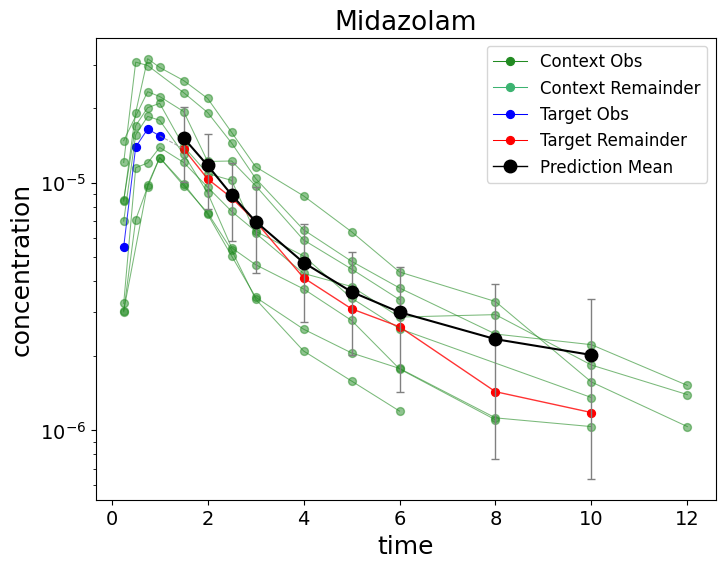
\includegraphics[width=\linewidth]{figures/midazolam_prediction.png}
        \caption{Midazolam}
        \label{fig:prediction_midazolam}
    \end{subfigure}
    \hfill
    \begin{subfigure}[t]{0.31\textwidth}
        \centering
        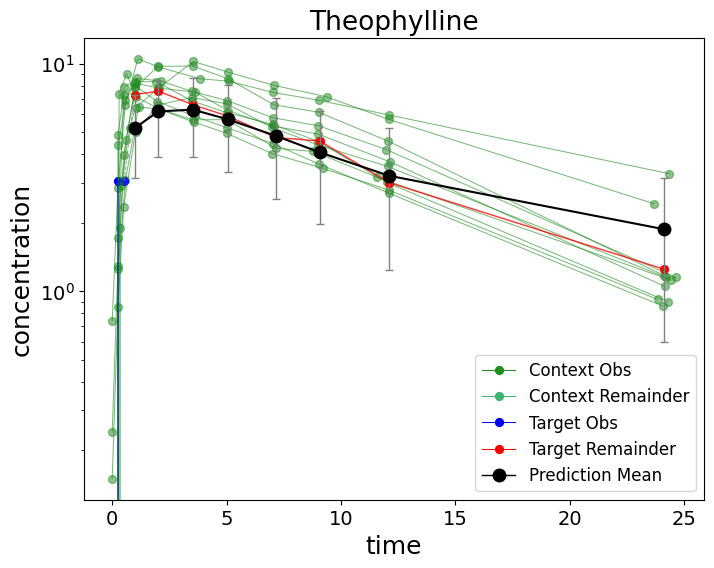
\includegraphics[width=\linewidth]{figures/theophylline_prediction.png}
        \caption{Theophylline}
        \label{fig:prediction_theophylline}
    \end{subfigure}
    \hfill
    \begin{subfigure}[t]{0.32\textwidth}
        \centering
        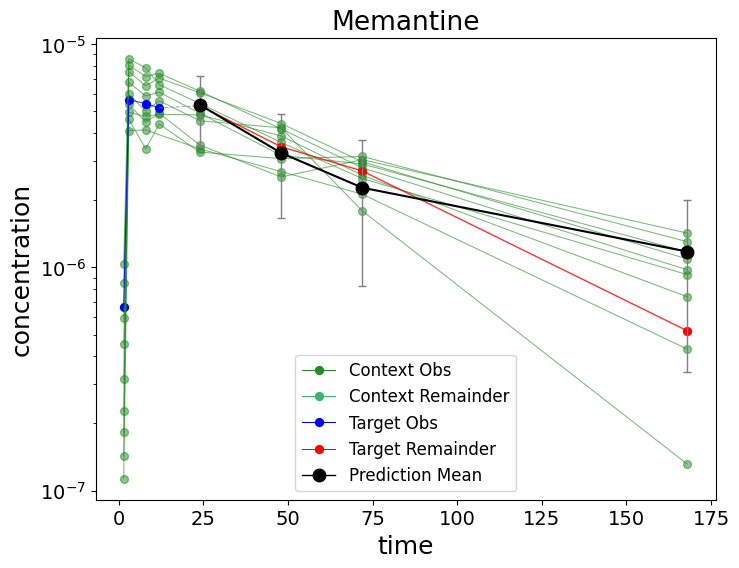
\includegraphics[width=\linewidth]{figures/memantine_prediction.png}
        \caption{Memantine}
        \label{fig:prediction_memantine}
    \end{subfigure}

    \caption{Predictive plots for three representative compounds. Conditioned on the population study context (green), the model uses the partial observations (blue) of a new patient to sample forecasts (red) from the predictive distribution, with the predictive mean (black) shown for reference.}
    \label{fig:prediction_row}
\end{figure*}


\subsection{Conditional Functional Flow Matching Model}
\label{sec:model-cffm}

We now instantiate the abstract conditional generation problem from Section~\ref{sec:preliminaries} in the PK setting, and describe the conditional flow-matching construction used by Prior-Fitted Functional Flows (\texttt{PFF}).
%
The key objects are: (i) a \emph{simulator-induced} target measure over concentration trajectories, and (ii) a single learnable vector field in function space whose induced flow maps a tractable reference measure to the target in zero-shot mode.
%
Crucially, \texttt{PFF} is trained once and used for both population synthesis and forecasting. 
%
The two modes differ only in the context provided at inference time, and in the corresponding choice of reference measure.

Thus, our methodology distinguishes two conditioning levels
\begin{enumerate}
\item \textit{Study-level conditioning} on $\mathcal S$, which is always present and encodes population variability and sampling patterns. In \texttt{PFF}, $\mathcal S$ enters the vector field via attention-based mechanisms.
\item \textit{Individual-level conditioning} on an optional prefix of measurements for a new individual.
%
When a prefix is available, \texttt{PFF} performs forecasting by transporting uncertainty only in the unobserved continuation. When no prefix is available, \texttt{PFF} reduces to population synthesis.
\end{enumerate}

Accordingly, we define a context space $\CM = \mathscr{S} \times \mathscr{O}$, 
%
where $\mathscr{S}$ denotes the set of studies, and $\mathscr{O}$ collects the information available for a new individual. 
%
In \textit{population synthesis} we take $\mathscr{O}=\{\varnothing\}$ (no individual measurements). 
%
In \textit{forecasting} we use a nontrivial element $o\in\mathscr{O}$ defined below.

\textbf{A new individual and prefix split}.
%
We distinguish the observed study $\mathcal S$ from a new \textit{virtual} individual $\mathcal D^{\rm n} = (\mathbf u^{\rm n},\boldsymbol{\tau}^{\rm n},\mathbf y^{\rm n})$,
%
for which we may observe a short prefix of measurements. 
%
We introduce a split index $p \in \{0,\dots,P\}$,
%
which partitions the observations into a revealed \textit{past} and an unobserved \textit{future}. Writing $\mathbf{y}^{\rm n}=(\mathbf y^{\rm n}_{\tt P},\mathbf y^{\rm n}_{\tt F})$ and $\boldsymbol{\tau}^{\rm n}=(\boldsymbol{\tau}^{\rm n}_{\tt P},\boldsymbol{\tau}^{\rm n}_{\tt F})$,
%
we define
\[
\mathbf y^{\rm n}_{\tt P}=(y_1^{\rm {\rm n}},\dots,y_p^{\rm n}),\quad
\mathbf y^{\rm n}_{\tt F}=(y_{p+1}^{\rm {\rm n}},\dots,y_{T_{\rm n}}^{\rm n}),
\]
and similarly for $\boldsymbol{\tau}^{\rm n}_{\tt P},\boldsymbol{\tau}^{\rm n}_{\tt F}$.  Setting $p=0$ corresponds to \text{population synthesis}, so $o=\varnothing$ and $c=(\mathcal S,\varnothing)$. For $p>0$, we perform \textit{forecasting}, with $o = (\mathbf u^{\rm n},\boldsymbol{\tau}^{\rm n}_{\tt P},\mathbf y^{\rm n}_{\tt P},p) \in \mathscr{O}$, and $c \;=\; (\mathcal S,o)\in\CM$. In what follows, we drop the superscript $n$ for new individuals whenever the meaning is clear from context.

\textbf{Past-future decomposition in function space}.
%
Let $\mathcal T=[0,T]$ and let $\F= C([0,T])$ be a Hilbert space of continuous concentration trajectories.
%
This choice reflects the physical fact that PK concentration trajectories are continuous in time, and it allows us to speak meaningfully about values at a split time.
%
For a given prefix length $p$, we define the split time $\tau_p$ and the corresponding intervals $\mathcal T_{\tt P}=[0,\tau_p]$, and $\mathcal T_{\tt F}=[\tau_p,T]$.
%
We represent the full trajectory as a pair
\[
f \equiv (f_{\tt P},f_{\tt F}),
\qquad
f_{\tt P}:\mathcal T_{\tt P}\to\mathbb R,
\qquad
f_{\tt F}:\mathcal T_{\F}\to\mathbb R,
\]
and we identify the full function space with the product $\F = \F_{\tt P}\times\F_{\tt F},$
%
where $\F_{\tt P}$ and $\F_{\tt F}$ are Hilbert spaces of functions on $\mathcal T_{\tt P}$ and $\mathcal T_{\tt F}$, respectively. 
%
To ensure the pair represents a single continuous trajectory, we impose compatibility at intersection, i.e., $f_{\tt P}(\tau_p) = f_{\tt F}(\tau_p)$.
%
Intuitively, $f_{\tt P}$ is the revealed prefix segment and $f_{\tt F}$ is the unobserved continuation.

What is more, we define $\tau_0 = 0$ so that, when $p=0$, the ``past'' interval collapses, and the ``future'' interval corresponds to the full domain. 
%
This makes population synthesis a special case of the same construction.

\textbf{Simulator-induced target measure}.

Our simulator $P^{\mathrm{sim}}$ first samples latent kinetic parameters (physics) and study designs (dosing, covariates, sampling times).
%
Based on these, it generates continuous concentration curves $f$ and compiles them into discrete studies $\mathcal{S}$ (which contain discrete observations of multiple curves).
%
Crucially, we cannot query the simulator to generate curves for a specific, pre-defined study $\mathcal{S}$; we are restricted to the studies it stochastically generates.
%
Our learning task is therefore to use generated joint pairs $(\mathcal{S}, f)$ to approximate the conditional measure $\nu^{\mathrm{sim}}(\,\cdot\mid \mathcal S)$, enabling us to generalize to arbitrary studies later.
To extend this framework to forecasting, where an individual is partially observed, we decompose the trajectory as $f=(f_{\tt P},f_{\tt F})$. This joint law defines the \textit{past marginal}
$\nu^{\mathrm{sim}}_{\tt P}(\,\cdot\mid\mathcal S)\ \in\ \PM(\F_{\tt P})$,
%
and a corresponding \textit{future conditional}  $\nu^{\mathrm{sim}}_{\tt F}(\,\cdot\mid\mathcal{S},f_{\tt P})\ \in\ \PM(\F_{\tt F}).$ Informally, $\nu^{\mathrm{sim}}_{\tt F}$ describes plausible continuations compatible with a given prefix $f_{\tt P}$.
%
In practice, accessing $f_{\tt P}$ directly is impossible, and the individual-level context enters through the observations $o = (\boldsymbol{\tau}^n_{\tt P},\mathbf y^n_{\tt P}, \mathbf{u}^n)$.
%
The ojective is to learn to sample from these target conditionals, i.e. $\nu^{\mathrm{sim}}(\cdot \mid \mathcal{S})$ for synthesis and $\nu^{\mathrm{sim}}_{\tt F}(\cdot \mid \mathcal{S}, o)$ for forecasting, for \textit{any} observed context.

%
%Our simulator $P^{\mathrm{sim}}$ defines a broad prior over physiologically plausible compartmental PK models and induces, for each study $\mathcal S$, a measure over full concentration functions for a new individual $\nu^{\mathrm{sim}}(\,\cdot\mid \mathcal S)\ \in\ \PM(\F)$.

%By sampling $f\sim \nu^{\mathrm{sim}}(\cdot\mid\mathcal S)$ and writing $f=(f_{\tt P},f_{\tt F})$, we obtain the induced joint measure
%
%$\nu^{\mathrm{sim}}_{\tt P, \tt F}(\,\cdot\mid\mathcal S)\ \in\ \PM(\F_{\tt P}\times\F_{\tt F})$.
%
%This joint law defines the \textit{past marginal}
%$\nu^{\mathrm{sim}}_{\tt P}(\,\cdot\mid\mathcal S)\ \in\ \PM(\F_{\tt P})$,
%
%and a corresponding \textit{future conditional} 
%\begin{equation}
%\nu^{\mathrm{sim}}_{\tt F}(\,\cdot\mid\mathcal{S},f_{\tt P})\ \in\ \PM(\F_{\tt F}),
%\end{equation}
%so that, informally, $\nu^{\mathrm{sim}}_{\tt F}$ describes plausible continuations compatible with a given prefix function $f_{\tt P}$ under the PK prior.
%
%In practice, we do \textit{not} provide $f_{\tt P}$ to the model directly when forecasting. 
%
%The individual-level context enters only through the discrete prefix observations $(\boldsymbol{\tau}^n_{\tt P},\mathbf y^n_{\tt P}, \mathbf{u}^n)$ contained in $o$.

\textbf{Reference measure (unified synthesis and forecasting)}.
%
To train a single model that covers both modes, we use a reference measure on $\F_{\tt F}$ that depends on whether a prefix is available.
Let $\mathrm{GP}_{\mathcal T_{\tt F}}(\cdot)$ denote a Gaussian-process prior on $\mathcal T_{\tt F}$, and let $\mathrm{GP}_{\mathcal T_{\tt F}}(\cdot\mid \mathbf u,\mathbf y_{\tt P})$ denote the corresponding GP posterior restricted to $\mathcal T_{\tt F}$.
We define
\begin{equation}
\eta_{\tt F}(\cdot\mid o, p)
:=
\begin{cases}
\mathrm{GP}_{\mathcal T_{\tt F}}\bigl(\,\cdot\mid \mathbf u,\mathbf y_{\tt P}\bigr)
&\text{if} \, \, \, \, p>0,\\[4pt]
\mathrm{GP}_{\mathcal T_{\tt F}}(\,\cdot)
&\text{if} \, \, \, \, p=0,
\end{cases}
\label{eq:reference-measure}
\end{equation}
such that $\eta_{\tt F}(\cdot\mid o, p)\in\PM(\F_{\tt F})$.
%
Thus, in population synthesis ($p=0$) the flow starts from a GP prior over full trajectories (since $\F_{\tt F}\equiv\F$), whereas in forecasting ($p>0$) it starts from a GP posterior that extrapolates from the observed prefix.
%
In both cases, we use the same trainable vector field conditioned on the study $\mathcal S$. 
%
The only additional change is whether the input includes an individual prefix, which alters the reference measure and the conditioning context.


\begin{algorithm}[t]
\caption{Training of Prior-Fitted Functional Flows}
\label{alg:pff-training}
\DontPrintSemicolon
\SetKwInOut{KwIn}{Input} \SetKwInOut{KwOut}{Return}

\KwIn{Simulator $P^{\mathrm{sim}}$, Network $v_\theta$, Step size $\eta$.}
\KwOut{Trained parameters $\theta$}

\While{not converged}{
    $(\mathcal{S}, \mathbf{y}^{\rm n}, \boldsymbol{\tau}^{\rm n}) \sim P^{\mathrm{sim}}$ \tcp*{Sample from Simulator}
    $p \sim \mathcal{U}\{0, \dots, |\boldsymbol{\tau}^{\rm n}|-1\}$ \tcp*{ Sample Split} $\mathbf{y}^{\rm n} \to (\mathbf{y}_{\tt P}, \mathbf{y}_{\tt F})$ and $\boldsymbol{\tau}^{\rm n} \to (\boldsymbol{\tau}_{\tt P}, \boldsymbol{\tau}_{\tt F})$ \tcp*{Partition Data}
   $c = (\mathscr{S},\mathbf{u}^{\rm n}, \boldsymbol{\tau}_{\tt P}, \mathbf{y}_{\tt P})$ \tcp*{Set Context}
    $\mathbf{x}_{\tt F} \sim \text{GP}(\boldsymbol{\tau}_{\tt F} \mid \mathbf{y}_{\tt P}, \boldsymbol{\tau}_{\tt P})$    \tcp*{Sample Reference}
    $\mathbf{z}_0 = (\mathbf{y}_{\tt P}, \mathbf{x}_{\tt F})$, 
    $\mathbf{z}_1 = (\mathbf{y}_{\tt P}, \mathbf{y}_{\tt F})$ \tcp*{Set Start and End}

    $t \sim \mathcal{U}(0,1)$, $\mathbf{z}_t \sim \mathcal{N}(t \mathbf{z}_1 + (1-t)\mathbf{z}_0, \sigma_{\min}^2 I)$\;
    
    $u_t = (\mathbf{0}, \mathbf{y}_{\tt F} - \mathbf{x}_{\tt F})$ \tcp*{Target Velocity}
    
    $\mathcal{L}(\theta) = \| \mathbf{M}_{\tt F} \odot (v_\theta(\mathbf{z}_t, t, \mathcal{S}) - u_t) \|^2$ \tcp*{Loss}
    
    $\theta \leftarrow \theta - \eta \nabla_\theta \mathcal{L}(\theta)$\;
}
\end{algorithm}

%\begin{algorithm}[t]
%\caption{Training of Prior Fitted Functional Flow Matching}
%\label{alg:tsflow-uncond}
%\DontPrintSemicolon
%\SetKwInOut{KwIn}{Input}
%\SetKwInOut{KwOut}{Return}

%\KwIn{meta prior $P^{sim}$, network $v^\theta$, step size $\eta$.}
%\KwOut{$v^\theta$}

%\While{not converged}{
%    $ (\mathbf y^{\rm n}_{\tt F}, \boldsymbol{\tau}^{\rm n}_{\tt F},\boldsymbol{\tau}^{\rm n}_{\tt P},\mathbf y^{\rm n}_{\tt P}, \mathbf{u}^{\rm n},\mathcal{S})  = (\mathbf y^{\rm n}_{\tt F}, \boldsymbol{\tau}^{\rm n}_{\tt F}, o,\mathcal{S}) \sim P^{sim}$\;
 
%    $ f_{\tt F} \sim \eta_{\tt F}(\cdot\mid o, p) \text{ \quad } \*x_{\tt F} = f_{\tt F}(\boldsymbol{\tau}^{\rm n}_{\tt F})  $\;
%    $(x_0,y) \leftarrow \mathrm{OT}(x_0,x_1)$\;
%    $t \sim \mathcal{U}(0,1)$\;
%    $\mathbf{z}_t \sim \mathcal{N}\!\bigl(t \, \*z_1+(1-t)\*z_0,\;\sigma_{\min}^2 I\bigr) $\;
%    $\mathcal{L}(\theta) \leftarrow \left\|
%\*M_p \odot v^\theta_t(\mathbf{z}_t, \mathcal{S})
%-
% (\mathbf{y}^n_{\tt F}-\mathbf{x}_{\tt F})
%\right\|^2$\;
%    $\theta \leftarrow \theta - \eta\,\nabla_\theta \mathcal{L}(\theta)$\;
%}
%\end{algorithm}

\textbf{Conditional flow matching for PK}.
%
The data generation process of Section~\ref{sec:pretraining-prior} yields samples $\mathcal{D}^{\rm n}, \mathcal{S} \sim P^{\mathrm{sim}}$. 
%
Let us now sample $p \sim \text{Uniform}(0, \dots, P)$ and introduce the \textit{finite-dimensional} flow variables 
%
$\mathbf{z}_0 = (\mathbf{y}_{\tt P}^{\rm n}, \mathbf{x}_{\tt F})$ and $\mathbf{z}_1 = (\mathbf{y}_{\tt P}^{\rm n}, \mathbf{y}^{\rm n}_{\tt F})$. 
%
Here $\mathbf{x}_{\tt F} = \left(f_{\tt F}(\tau_{p+1}^{\rm n}), \dots, f_{\tt F}(\tau_{T_{\rm n}}^{\rm n}) \right)$, where $f_{\tt F} \sim \eta_{\tt F}$ is sampled from the reference measure (Eq.~\ref{eq:reference-measure}).

Similar to Eq.~\ref{eq:fm-cond-path}, we now introduce the (finite-dimensional) Gaussian conditional path 
\begin{equation}
\*z_t \sim p_t(\*z \mid \*z_0, \*z_1) =\mathcal{N}\!\bigl(t \, \*z_1+(1-t)\*z_0,\;\sigma_{\min}^2 I\bigr),
\end{equation}
and the associated target, triangular vector field
$
v_t(\*z \mid \*x_{\tt F},\*y_{\tt F}^{\rm n}) = (\mathbf{0}, \mathbf{y}_{\tt F}^{\rm n}- \mathbf{x}_{\tt F}).
$
Using this construction, we train a neural operator vector field
$v^\theta_t(\mathbf{z}, c)$ by minimizing the conditional flow matching loss
\begin{equation*}
\mathcal{L}(\theta)
=
\mathbb{E}_{t,p,\mathbf{x}_{\tt F},\mathbf{y}^{\rm n}_{\tt F}}
\!\left[
\left\|
\*M_p \odot v^\theta_t(\mathbf{z}_t, c)
-
 (\mathbf{y}^{\rm n}_{\tt F}-\mathbf{x}_{\tt F})
\right\|^2
\right],
\end{equation*}
where $\*M_p$ is a prefix-dependent mask that zeros out the ``past'' of the learnable vector field.


\begin{table*}[t]
    \centering
    \caption{\textbf{Comparison of Log-RMSE Across Models.}
    For each compound, we report mean log-RMSE with standard deviation in parentheses.
    The best-performing model for each compound is highlighted in \textbf{bold}.}
    \label{tab:main_results}
    \setlength{\tabcolsep}{3pt}
    \renewcommand{\arraystretch}{0.90}
    \smaller
    \begin{tabularx}{\textwidth}{l YYYYY}
        \toprule
        \textbf{Compound} & \textbf{NLME} & \textbf{Transf.} & \textbf{NODE} & \textbf{AICMET} & \textbf{PFF} \\
        \midrule
\rowcolor{lightochre}
caffeine & $0.294 \pm 0.294$ & $0.451 \pm 0.258$ & $0.432 \pm 0.209$ & $0.399 \pm 0.205$ & $\mathbf{0.174 \pm 0.086}$ \\
dextromethorphan & $0.752 \pm 0.752$ & $\mathbf{0.395 \pm 0.163}$ & $0.605 \pm 0.248$ & $0.595 \pm 0.364$ & $0.963 \pm 0.426$ \\
\rowcolor{lightochre}
digoxin & $\mathbf{0.300 \pm 0.300}$ & $0.683 \pm 0.242$ & $0.661 \pm 0.315$ & $0.691 \pm 0.464$ & $0.375 \pm 0.216$ \\
indometacin & $0.582 \pm 0.582$ & $0.429 \pm 0.328$ & $0.350 \pm 0.291$ & $0.536 \pm 0.203$ & $\mathbf{0.245 \pm 0.170}$ \\
\rowcolor{lightochre}
memantine & $\mathbf{0.343 \pm 0.343}$ & $0.513 \pm 0.335$ & $0.554 \pm 0.386$ & $0.475 \pm 0.341$ & $0.404 \pm 0.388$ \\
midazolam & $0.596 \pm 0.596$ & $0.288 \pm 0.173$ & $0.352 \pm 0.224$ & $\mathbf{0.264 \pm 0.151}$ & $0.295 \pm 0.300$ \\
\rowcolor{lightochre}
omeprazole & $1.300 \pm 1.300$ & $0.842 \pm 0.400$ & $1.003 \pm 0.618$ & $0.936 \pm 0.942$ & $\mathbf{0.593 \pm 0.161}$ \\
paracetamol & $\mathbf{0.299 \pm 0.299}$ & $0.447 \pm 0.274$ & $0.582 \pm 0.302$ & $0.352 \pm 0.187$ & $0.309 \pm 0.220$ \\
\rowcolor{lightochre}
repaglinide & $0.479 \pm 0.479$ & $0.709 \pm 0.268$ & $0.693 \pm 0.290$ & $\mathbf{0.339 \pm 0.311}$ & $0.681 \pm 0.155$ \\
rosuvastatin & $\mathbf{0.383 \pm 0.383}$ & $0.502 \pm 0.205$ & $0.535 \pm 0.303$ & $0.558 \pm 0.286$ & $0.495 \pm 0.336$ \\
\rowcolor{lightochre}
theophylline & $0.732 \pm 0.732$ & $0.356 \pm 0.141$ & $0.327 \pm 0.144$ & $0.274 \pm 0.109$ & $\mathbf{0.184 \pm 0.110}$ \\
tolbutamide & $0.723 \pm 0.723$ & $0.678 \pm 0.339$ & $0.578 \pm 0.263$ & $0.517 \pm 0.254$ & $\mathbf{0.421 \pm 0.214}$ \\
\rowcolor{lightochre}
1-hydroxy-midazolam &  & $0.567 \pm 0.327$ & $0.737 \pm 0.381$ & $0.491 \pm 0.309$ & $\mathbf{0.422 \pm 0.205}$ \\
4-hydroxy-tolbutamide &  & $0.354 \pm 0.174$ & $0.353 \pm 0.182$ & $0.335 \pm 0.164$ & $\mathbf{0.293 \pm 0.153}$ \\
\rowcolor{lightochre}
5-hydroxy-omeprazole &  & $1.286 \pm 0.472$ & $1.474 \pm 0.745$ & $1.188 \pm 0.451$ & $\mathbf{1.026 \pm 0.356}$ \\
dextrorphan &  & $0.733 \pm 0.445$ & $0.834 \pm 0.284$ & $\mathbf{0.563 \pm 0.287}$ & $0.585 \pm 0.487$ \\
\rowcolor{lightochre}
hydroxy-repaglinide &  & $0.069 \pm 0.217$ & $\mathbf{0.049 \pm 0.156}$ & $0.076 \pm 0.240$ & $0.070 \pm 0.221$ \\
omeprazole sulfone &  & $\mathbf{1.054 \pm 0.297}$ & $1.390 \pm 0.488$ & $1.082 \pm 0.509$ & $1.156 \pm 0.355$ \\
\rowcolor{lightochre}
paracetamol glucuronide &  & $0.357 \pm 0.192$ & $0.297 \pm 0.169$ & $0.307 \pm 0.184$ & $\mathbf{0.265 \pm 0.114}$ \\
paraxanthine &  & $0.413 \pm 0.181$ & $0.287 \pm 0.135$ & $0.312 \pm 0.138$ & $\mathbf{0.273 \pm 0.143}$ \\
\bottomrule
\end{tabularx}
\end{table*}

\textbf{Vector-field parameterization}.
%
We parameterize the transport through a time-dependent triangular velocity field $v^{\theta}:\ [0,1]\times \mathscr{S} \times \F_{{\tt F}} \to \F_{{\tt F}}$. The model is an \emph{operator encoder--decoder transformer} that mirrors the standard sequence-to-sequence architecture of \citep{vaswani2017attention}. A \emph{context encoder} maps the context $\mathscr{C}$ to a set of subject-level representations using multi-head self-attention, with block-diagonal masking to prevent information flow across subjects. A \emph{target decoder} takes the flow-interpolated target individual $\mathbf{z}_t$ and applies non-causal self-attention over its past and future representations, followed by cross-attention blocks over the study-encoder outputs. The observation times are treated as positional encoding. One key departure from the standard transformer architecture is that both encoder and decoder operate on discretized functions over observation times that are subject-specific and not aligned to a common regular time grid. All attention operations are therefore replaced by their \emph{continuum operator} counterparts \citep{calvello2024continuum}, which correct for the grid irregularities via a trapezoidal quadrature approximation. For further details on the architecture see appendix~\ref{app:architecture}.
 

\begin{figure}[t]
    \centering
    \begin{minipage}[b]{0.4\textwidth}
        \centering
        (a)
            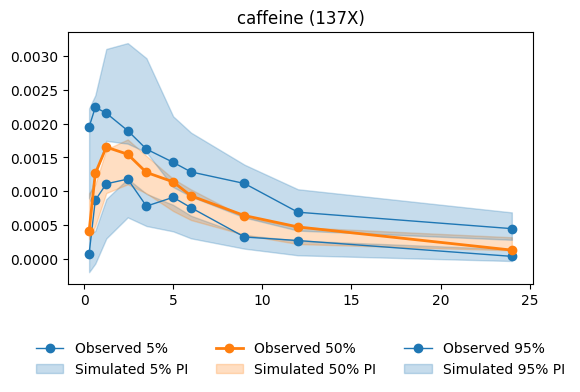
\includegraphics[width=\linewidth]{figures/caffeine_vpc.png}
    \end{minipage}
    \hfill
    \begin{minipage}[b]{0.4\textwidth}
        \centering
        (b)
            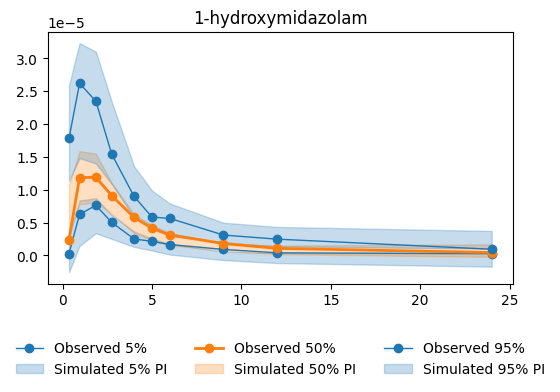
\includegraphics[width=\linewidth]{figures/1_hydroxymidazolam_vpc.png}
    \end{minipage}
    \caption{Visual predictive checks (VPCs) for (a) caffeine and (b) 1-hydroxy-midazolam. Each panel compares observed concentrations to simulation-derived prediction intervals.}
    \label{fig:vpc_only}
\end{figure}

 %\subsection{Inference via Conditional OT Flow Matching}
% Similar to \cite{dutordoir2023neural} we model the marginals and conditionals of $\nu^s$ by {\color{red}[ could be preciser here. $\nu^s$ has not been defined? and (13) refers to the marginals or to the conditionals?]}:
%\begin{equation}
% p(\mathbf{Y}^n \mid \mathcal{S}, \mathbf{u}^n, \boldsymbol{\tau}^n) = \int p(\mathbf{Y}^n \mid \mathcal{S}, \mathbf{u}^n, \boldsymbol{\tau}^n, f)\nu^s(df) ,
% \end{equation}
%where $\mathcal{S}$ denotes the study-level dataset, and
% $(\mathbf{u}^n, \boldsymbol{\tau}^n)$ represent the dosing information and observation
% times of the new individual. Notice that the functional aspect of the data generation is achieved by conditioning on the times where the observation is expected $\boldsymbol{\tau}^n$. Finally, we place a measure on the input space $\mu_{\boldsymbol{\tau}} \in \PM(\mathcal{T})$ {\color{red}[unclear what $\mathcal{T}$ is, see above]} and denote $\*Y^n \sim P_1$ with the procedure $\boldsymbol{\tau}^n \sim \mu_{\boldsymbol{\tau}}$, $f^n \sim \nu^s()$ and we evaluate $\*Y^n = f^n(\boldsymbol{\tau}) = (f(\tau^n_1),f(\tau^n_2),...,f(\tau^n_T))$.

% \subsection{Prior Fitted Functional Flows}
% We first introduce the \textit{flow variable} $\*X_t$\footnote{notice that $t$ corresponds to the flow time, whereas $\tau$ corresponds to the input time of the observed functions}
% \[
% \mathbf{X}^p_t=(\mathbf{y}_p,\mathbf{x}_t),\quad
% \mathbf{X}^p_0=(\mathbf{y}_p,\mathbf{x}^f_0),\quad
% \mathbf{X}^p_1=(\mathbf{y}_p,\mathbf{y}_f),
% \]
% Where $\*X^p_t \in \mathbb{R}^T$ and $\*x^p_t \in \mathbb{R}^{T-p}$ {\color{red}[there is no $x_t^p$ above]}. The lower case indicates the section of the time series that corresponds unobserved future. We also define the future mask $\*F^p = (\*0, \*M^p_f) {\color{red} \in ?}$, which zeros out all the past of the vector. This construction allows us to define a triangular vector field, that is conditioned on all the observations $\*Y^n$ but leaves the conditioning part of the flow untouched.
% \subsection{Bridge Construction}
% With the previous notations we can construct the interpolations such that 
% \begin{equation}
% p_t(\*x \mid \*x_0,\*y_f)=\mathcal{N}\!\bigl(t\*y^f+(1-t)\*x_0,\;\sigma_{\min}^2 I\bigr)
% \end{equation}
% {\color{red}[(14) is not a bridge technically speaking (for this $\sigma_min$ would need to be timedependent such that it is zero at the endpoints)]} and the associated endpoint-conditioned vector field is given by
% \begin{equation}
% u_t(\mathbf{X} \mid \mathbf{X}_0, \mathbf{X}_1, c)
% = \mathbf{X}_1 - \mathbf{X}_0.
% \end{equation}

% \textbf{Training Objective}
% Using this construction, we train the neural vector field
% $v_t(\mathbf{X}, \mathcal{C}; \theta)$ by minimizing the conditional flow matching loss
% \begin{equation}
% \mathcal{L}_{\mathrm{CFM}}(\theta)
% =
% \mathbb{E}_{t,p,\mathbf{X}^p_0,\mathbf{X}^p_1}
% \!\left[
% \left\|
% \*F^p_t \odot v_t(\mathbf{X}^p_t, \mathcal{C}; \theta)
% -
% \*F^p_t \odot (\mathbf{X}^p_1-\mathbf{X}^p_0)
% \right\|^2
% \right],
% \end{equation}
% {\color{red}[there probably should be no $t$ in the mask?]}






% \subsection{Gaussian Process Regression for Noise}\label{sec:gp_priors}
% Since $q_0(\*x_0)$ is a GP, we can compute $q_0(\*x_0 \mid \*Y^{p})$ analytically [{\color{red} there is no $Y^p$ yet?}].
% We begin by factorizing the conditional prior as
% \[
% q_0(\*X_0 \mid \*Y^{p})
% \;=\;
% q_0(\*x_0^{p}\mid \*y_{p})\,
% q_0(\*x_0^{f}\mid \*y_{p}),
% \]
% which follows by assuming conditional independence of $\*x_0^{p}$ and $\*x_0^{f}$ given $\*y^{p}$.
% We choose $
% q_0(\*x_0^{p}\mid \*y_{p}) \;=\; \delta(\*x_0^{p}-\*y_{p})
% $ to retain the information from the observation.
% For the unobserved future part, we employ Gaussian process regression (GPR) to model the conditional distribution.
% Specifically,
% \begin{equation}
% q_0(\*x_0^{f}\mid \*Y^{p})
% \;=\;
% \mathcal{N}\!\bigl(\*x_0^{f}\mid \mu_{f\mid p}, \Sigma_{f\mid p}\bigr),
% \label{eq:gpr-cond}
% \end{equation}
% where $\mu_{f\mid p}=\Sigma_{fp}\Sigma_{pp}^{-1}\*Y^{p}$ and $\Sigma_{f\mid p}=\Sigma_{ff}-\Sigma_{fp}\Sigma_{pp}^{-1}\Sigma_{pf}$, with covariance blocks computed from the kernel $K$ evaluated at the input time grids $\boldsymbol{\tau}^n=(\boldsymbol{\tau}_p^n,\boldsymbol{\tau}_f^n)$, namely $\Sigma_{pp}=K(\boldsymbol{\tau}_p^n,\boldsymbol{\tau}_p^n)$, $\Sigma_{ff}=K(\boldsymbol{\tau}_f^n,\boldsymbol{\tau}_f^n)$, $\Sigma_{fp}=K(\boldsymbol{\tau}_f^n,\boldsymbol{\tau}_p^n)$, and $\Sigma_{pf}=K(\boldsymbol{\tau}_p^n,\boldsymbol{\tau}_f^n)$.


% You can also try: \SetCommentSty{scriptsize}
